\documentclass{article}
\usepackage{geometry}
\usepackage{titling}
\usepackage{hyperref}
\usepackage{amsmath}
\usepackage{amssymb}
\usepackage{graphicx}
\usepackage[dvipsnames]{xcolor}

\geometry{
  a4paper,
  total = {170mm, 257mm},
  left = 20mm,
  top = 20mm,
}
\graphicspath{ {./images/} }

\title{Trabajo práctico N° 2}
\author{Emanuel Nicolás Herrador}
\date{Marzo 2025}

\makeatletter
\def\@maketitle{%
  \newpage
  \null
  \vskip 1em%
  \begin{center}%
  \let \footnote \thanks
    {\LARGE \@title \par}%
    \vskip 1em%
    {\large \@date}%
  \end{center}%
  \par
  \vskip 1em}
\makeatother

\begin{document}

\maketitle

\noindent\begin{tabular}{@{}ll}
	Estudiante & \theauthor \\
\end{tabular}

\section*{Ejercicio 1}
Los capítulos 4, 5 y 10 se encuentran resumidos en la tercer clase.

\section*{Ejercicio 2}
El problema es el clásico de lectores y escritores, con la condición de que puede haber o bien solo a lo sumo $K$ lectores o bien solo a lo sumo $1$ escritor.

El esquema que se quiere plantear es el siguiente:
\begin{figure}[ht]
	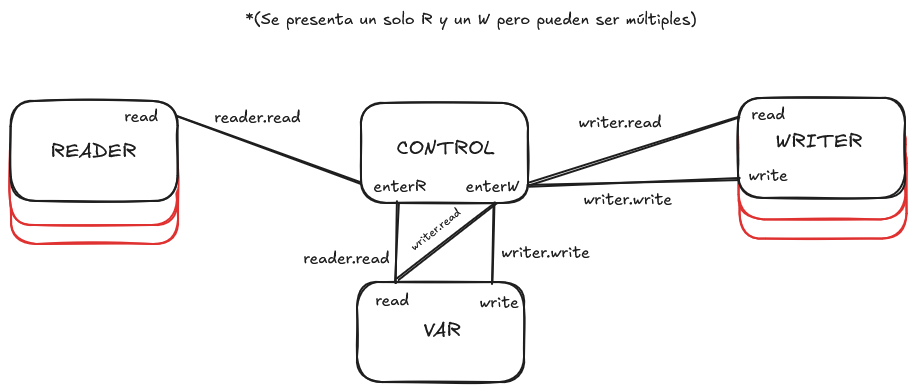
\includegraphics[width=0.9\textwidth]{02-02.png}
	\centering
\end{figure}

Cuyo diagrama FSP se corresponde a:
\begin{verbatim}
  const N = 3 
  const M = 3 
  const K = 2 

  VAR = (read -> VAR | write -> VAR).

  PERSON (AN=2) = (action[i:1..AN] -> PERSON).

  CONTROL = CONTROL[0][0],
  CONTROL[r:0..N][w:0..1] = (when(!r && !w) enterW -> CONTROL[r][w+1]
                            |when(r < K && !w) enterR -> CONTROL[r+1][w]
                            |when(w) exitW -> CONTROL[r][w-1]
                            |when(r) exitR -> CONTROL[r-1][w]
                            ).

  ||READWRITE_SYSTEM = (reader[1..N]:PERSON(1) || writer[1..M]:PERSON(2)
                                               || control:CONTROL || var:VAR)
                      /{reader.read/reader[1..N].action[1],
                        writer.read/writer[1..M].action[1],
                        writer.write/writer[1..M].action[2],

                        reader.read/control.enterR,
                        writer.{read, write}/control.enterW,

                        {reader, writer}.read/var.read,
                        writer.write/var.write
                        }
                      @{reader.read, writer.{read, write}}.
\end{verbatim}

\section*{Ejercicio 3}
En este ejercicio hay varios empleados, varias terminales y una sola central.
En particular, las dos operaciones destacadas son consulta y reserva (lectura y escritura).
Algo observable es que el problema es igual al anterior, permitiendo varios lectores en simultáneo pero solo un escritor.
La única diferencia es que en vez de cambiar una sola variable, es una por cada asiento del teatro.

Teniendo esto en cuenta, la idea de la solución es similar a la anterior, solo que no hace falta que implementemos un monitor porque la cantidad de lectores no tiene límite.
Simplemente, lo que podemos hacer es un lock para cuando alguien quiera reservar un asiento y evitar que se realice una reserva de un asiento ya reservado.

Notar que va a haber lecturas incorrectas por parte de los empleados a veces, pero esto tiene sentido porque implementar un lock que encapsule tanto a consulta y reserva no cumpliría con los requerimientos.
Esto es así dado que considero que las acciones son totalmente separadas en el tiempo y hacerlas atómicas sería una gran ineficiencia en el sistema.
En el caso de una lectura incorrecta, esto se soluciona no permitiendo reservar algo ya reservado.
Es decir, otro empleado "te puede ganar el asiento" si lo reserva antes que vos.

El diagrama de la estructura pensada es el siguiente:
\begin{figure}[ht]
	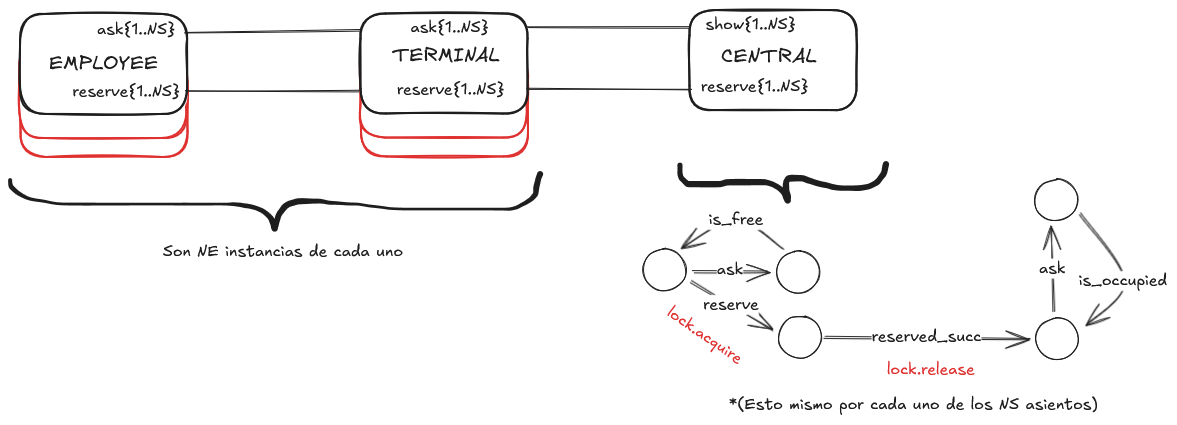
\includegraphics[width=1\textwidth]{02-03.png}
	\centering
\end{figure}

Y la definición del modelo en  FSP es:
\begin{verbatim}
  const NE = 2
  const NS = 3

  LOCK = (acquire -> release -> LOCK).

  EXTERNAL = (ask[1..NS] -> EXTERNAL | reserve[1..NS] -> EXTERNAL).

  SEAT = SEAT[0],
  SEAT[i:0..1] = (when(!i) show -> is_free -> SEAT[i]
                 |when(!i) reserve -> reserved_successfully -> SEAT[1]
                 |when(i) show -> is_occupied -> SEAT[i]
                 ).

  ||THEATER_SYSTEM = ({employee, terminal}[1..NE]:EXTERNAL || central[1..NS]:SEAT
                                                           || lock[1..NS]:LOCK)
                     /{ask[i:1..NS]/{{employee, terminal}[1..NE].ask[i], central[i].show},
                       reserve[i:1..NS]/{{employee, terminal}[1..NE].reserve[i],
                                         central[i].reserve},
                       
                       reserve[i:1..NS]/lock[i].acquire,
                       reserved_successfully[i:1..NS]/{lock[i].release,
                                                       central[i].reserved_successfully}
                      }
                     @{{ask, reserve}[1..NS]}.
\end{verbatim}

\section*{Ejercicio 4}
Este ejercicio es un caso donde el recurso compartido solo puede ser usado por una persona a la vez, sea el cocinero o un salvaje que se esté sirviendo de la olla.
Es decir, supongo que la olla no es tan grande como para permitir que varias personas se sirvan a la vez.
Aclarado lo anterior, al ser simple el diagrama de estructura, directamente paso al modelado en FSP:
\begin{verbatim}
  const M = 5

  POT = POT[M],
  POT[i:0..M] = (when(i) serve -> serve_complete -> POT[i-1]
                |when(!i) refill -> refill_complete -> POT[M]
                ).

  SAVAGE = SAVAGE[0],
  SAVAGE[i:0..1] = (when(i) eat -> SAVAGE[0]
                    |when(!i) get_food -> SAVAGE[1]
                    ).

  COOK = (refill -> COOK).

  LOCK = (acquire -> release -> LOCK).

  ||TRIBE = (savage[1..3]:SAVAGE || chef:COOK || pot:POT || lock:LOCK)
            /{savage[1..3].get_food/{pot.serve, lock.acquire},
              chef.refill/{pot.refill, lock.acquire},

              pot.{serve_complete, refill_complete}/lock.release
             }
            @{savage[1..3].{get_food, eat}, chef.refill}.
\end{verbatim}

\section*{Ejercicio 5}
Podemos notar que la idea de este canal es similar a la utilizada con anterioridad en los ejercicios 11, 12 y 13 del práctico anterior en la cinta.
Como en sí no nos importa modelar el orden de los mensajes acá, podemos considerar la definición de buffer que solo toma en cuenta la cantidad.

Por ello mismo, el modelo es el siguiente:
\begin{verbatim}
  PERSON = (action -> PERSON).

  BUFFER (BN=2) = BUFFER[0],
  BUFFER[i:0..BN] = (when(i < BN) put -> BUFFER[i+1]
                    |when(i > 0) get -> BUFFER[i-1]
                    ).

  ||SYSTEM = ({producer, consumer}:PERSON || buffer:BUFFER(4))
             /{make/{producer.action, buffer.put},
               use/{consumer.action, buffer.get}
               }.
\end{verbatim}

\section*{Ejercicio 6}
El protocolo que se debe modelar es el siguiente:
\begin{figure}[ht]
	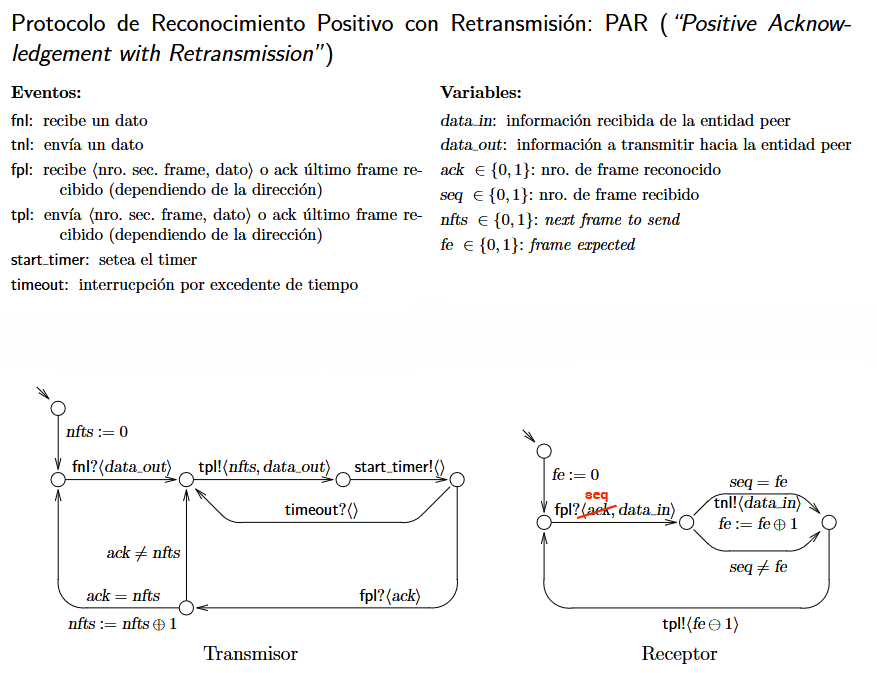
\includegraphics[width=0.8\textwidth]{02-06.png}
	\centering
\end{figure}

Y el modelo propuesto en FSP es:
\begin{verbatim}
  range BIT = 0..1

  TRANSMITTER = TRANSMITTER[0],
  TRANSMITTER[nfts:BIT] = (fnl -> SEND_FRAME[nfts]),
  SEND_FRAME[nfts:BIT] = (tpl[nfts] -> start_timer -> 
                              (timeout -> SEND_FRAME[nfts]
                              |fpl[ack:BIT] -> if(ack != nfts) then SEND_FRAME[nfts]
                                                               else TRANSMITTER[!nfts]
                              )
                         ).

  RECEIVER = RECEIVER[0],
  RECEIVER[fe:BIT] = (fpl[seq:BIT] ->
                              if(seq == fe) then (tnl -> tpl[fe] -> RECEIVER[!fe])
                                            else (tpl[!fe] -> RECEIVER[fe])
                     ).

  CHANNEL = (tpl[i:BIT] -> CHANNEL_SEND[i]),
  CHANNEL_SEND[i:BIT] = (fpl[i] -> CHANNEL 
                        |fpl[i] -> CHANNEL_SEND[i]        // Duplicate 
                        |lost -> CHANNEL                  // Lost     
                        ).

  ||PAR = (transmitter:TRANSMITTER || receiver:RECEIVER || channel[0..1]:CHANNEL)
          /{transmitter.tpl[i:BIT]/channel[0].tpl[i],
            receiver.tpl[i:BIT]/channel[1].tpl[i],

            transmitter.fpl[i:BIT]/channel[1].fpl[i],
            receiver.fpl[i:BIT]/channel[0].fpl[i]
           }
          \ {transmitter.{start_timer, timeout},
             channel[BIT].lost
            }.
\end{verbatim}

\section*{Ejercicio 7}
El protocolo que se debe modelar es el siguiente:
\begin{figure}[ht]
	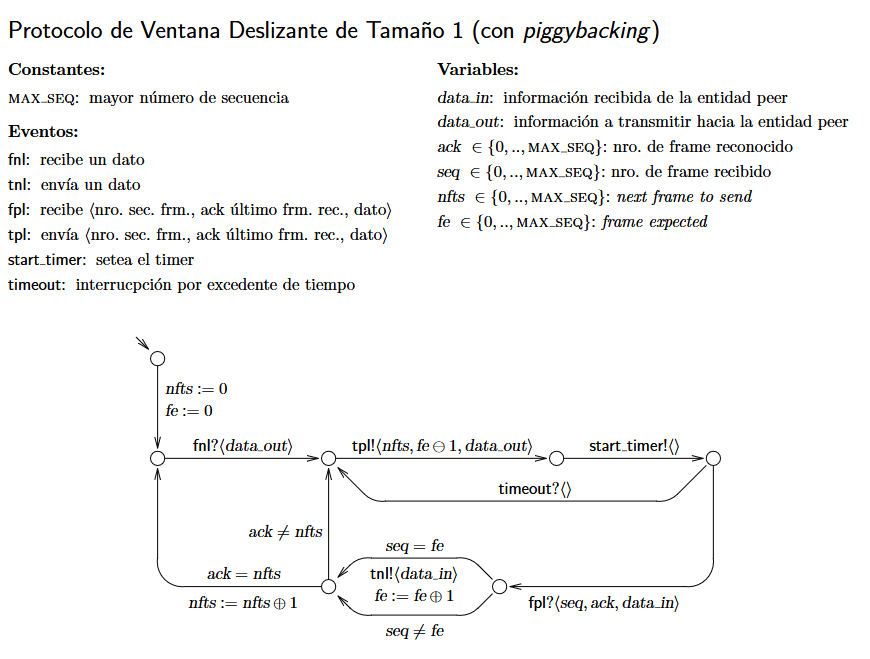
\includegraphics[width=0.8\textwidth]{02-07.png}
	\centering
\end{figure}

Y el modelo propuesto en FSP es:
\begin{verbatim}
  const MAX_SEQ = 1
  range R = 0..MAX_SEQ

  DEVICE = DEVICE[0][0],
  DEVICE[ntfs:R][fe:R] = (fnl -> SEND[ntfs][fe]),
  SEND[ntfs:R][fe:R] = (tpl[ntfs][(fe+1) % (MAX_SEQ+1)] -> start_timer -> 
                            (timeout -> SEND[ntfs][fe]
                            |fpl[seq:R][ack:R] -> 
                                if(seq != fe) then PREPARE[ntfs][fe][ack]
                                              else PREPARE[ntfs][(fe+1) % (MAX_SEQ+1)][ack]
                            )
                       ),
  PREPARE[ntfs:R][fe:R][ack:R] = if(ack != ntfs) then SEND[ntfs][fe]
                                                 else DEVICE[(ntfs+1) % (MAX_SEQ+1)][fe].

  CHANNEL = (tpl[i:R][j:R] -> (fpl[j][i] -> CHANNEL
                              |lost -> CHANNEL 
                              )
            ).

  ||PROTOCOL = ({transmitter, receiver}:DEVICE || channel[0..1]:CHANNEL)
               /{transmitter.tpl[i:R][j:R]/channel[0].tpl[i][j],
                 receiver.tpl[i:R][j:R]/channel[1].tpl[i][j],

                 transmitter.fpl[i:R][j:R]/channel[1].fpl[i][j],
                 receiver.fpl[i:R][j:R]/channel[0].fpl[i][j],

                 channel[0..1].lost/{transmitter, receiver}.timeout
                }
              \ {{transmitter, receiver}.{start_timer, timeout},
                 channel[0..1].lost 
                }.
\end{verbatim}
% TODO: Esperar a la respuesta del profe 
\begin{quotation}
	\textbf{\textcolor{red}{Nota:}} En este caso tiene un problema de liveness. Esperar a la respuesta del profe para completarlo.
\end{quotation}

\section*{Ejercicio 8}
% TODO: Terminar
\begin{quotation}
	\textbf{\textcolor{red}{Nota:}} Antes de hacer este ejercicio, completar el 8.
\end{quotation}

\section*{Ejercicio 9}
El diagrama de estructura a considerar es:
\begin{figure}[!htb]
	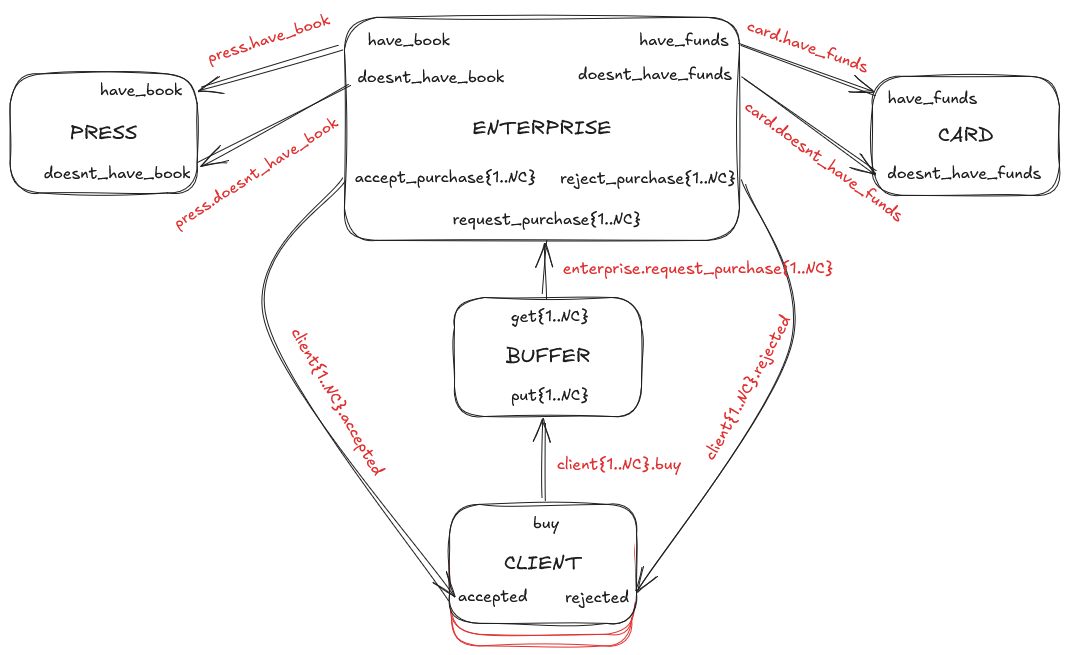
\includegraphics[width=0.9\textwidth]{02-09.png}
	\centering
\end{figure}

Con ello, el modelo de este problema es el siguiente:
\begin{verbatim}
  const NC = 2 
  
  BUFF (NT=2) = (put[obj:1..NT] -> get[obj] -> BUFF).
  ||BUFFER (BN=2, NT=2) = ([1..BN]:BUFF(NT))
                          /{put[obj:1..NT]/[1].put[obj],
                            [i:2..BN].put[obj:1..NT]/[i-1].get[obj],
                            get[obj:1..NT]/[BN].get[obj]
                           }
                          @{{put, get}[obj:1..NT]}.

  CLIENT = (buy -> (accepted -> CLIENT | rejected -> CLIENT)).

  NERD_PRESS = (have_book -> NERD_PRESS | doesnt_have_book -> NERD_PRESS).

  PLASTI_CARD = (have_funds -> PLASTI_CARD | doesnt_have_funds -> PLASTI_CARD).

  ENTERPRISE = (request_purchase[id:1..NC] -> 
                    (have_book -> (have_funds -> accept_purchase[id] -> ENTERPRISE
                                  |doesnt_have_funds -> reject_purchase[id] -> ENTERPRISE
                                  )
                    |doesnt_have_book -> reject_purchase[id] -> ENTERPRISE
                    )
               ).

  ||SYSTEM = (client[1..NC]:CLIENT || buffer:BUFFER(2, 2) || press:NERD_PRESS
                                   || card:PLASTI_CARD || enterprise:ENTERPRISE)
             /{client[id:1..NC].buy/buffer.put[id],
               enterprise.request_purchase[id:1..NC]/buffer.get[id],

               client[id:1..NC].accepted/enterprise.accept_purchase[id],
               client[id:1..NC].rejected/enterprise.reject_purchase[id],

               card.have_funds/enterprise.have_funds,
               card.doesnt_have_funds/enterprise.doesnt_have_funds,
               press.have_book/enterprise.have_book,
               press.doesnt_have_book/enterprise.doesnt_have_book
              }.
\end{verbatim}

\section*{Ejercicio 10}
El diagrama de estructura en el que me basé es el siguiente:
\begin{figure}[!htb]
	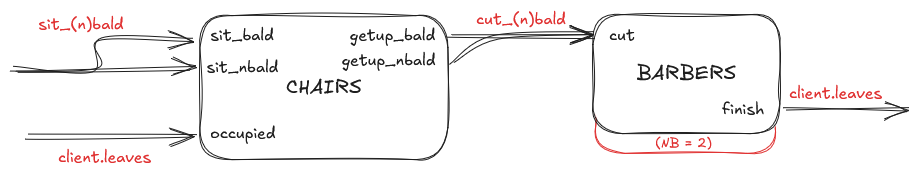
\includegraphics[width=0.8\textwidth]{02-10.png}
	\centering
\end{figure}

Y, por ello, el modelo elegido es:
\begin{verbatim}
  BARBER = (cut -> finish -> BARBER).

  CHAIRS (NC=3) = CHAIRS[0][0],
  CHAIRS[bald:0..NC][nbald:0..NC] =
                      (when(bald + nbald == NC) occupied -> CHAIRS[bald][nbald]
                      |when(bald + nbald < NC) sit_bald -> CHAIRS[bald+1][nbald]
                      |when(bald + nbald < NC) sit_nbald -> CHAIRS[bald][nbald+1]
                      |when(bald) getup_bald -> CHAIRS[bald-1][nbald]
                      |when(!bald && nbald) getup_nbald -> CHAIRS[bald][nbald-1]
                      ).

  ||SYSTEM = (barbers[1..2]:BARBER || chairs:CHAIRS(3))
             /{client_leaves/{chairs.occupied, barbers.finish},
               barbers[i:1..2].{cut_bald, cut_nbald}/barbers[i].cut,
               barbers[1..2].cut_bald/chairs.getup_bald,
               barbers[1..2].cut_nbald/chairs.getup_nbald
              }.
\end{verbatim}

\pagebreak
\section*{Ejercicio 11}
Tenemos el siguiente diagrama de los dos sistemas:
\begin{figure}[ht]
	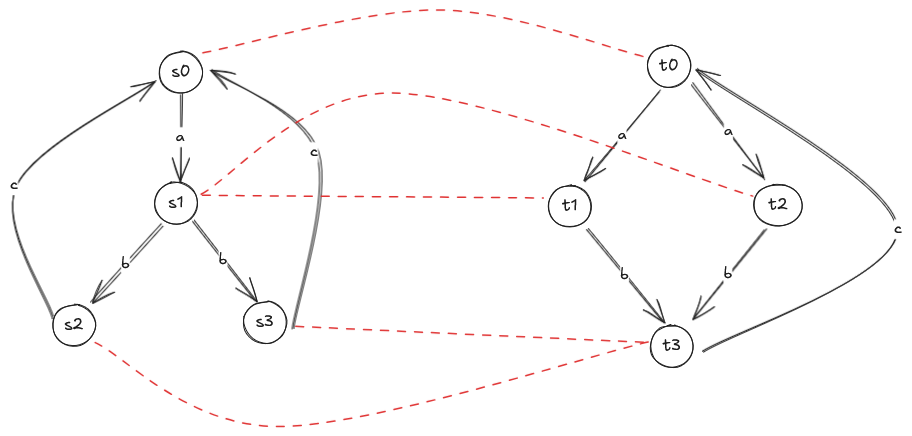
\includegraphics[width=0.8\textwidth]{02-11.png}
	\centering
\end{figure}

Se observa que $R = \{(s_0, t_0), (s_1, t_1), (s_1, t_2), (s_2, t_3), (s_3, t_3)\}$ es una bisimulación porque tanto $R$ como $R^{-1}$ son simulaciones.

\section*{Ejercicio 12}
Cuando hacemos las dos minimizaciones, podemos observar que la minimización sin reducción de $\tau$ tiene exactamente el mismo grafo que el original.
Es decir, son isomorfas por lo que obviamente son bisimilares débilmente.

Respecto a la primer minimización con reducción de $\tau$ activada, se observa el siguiente diagrama (en comparación con el original):
\begin{figure}[!htb]
	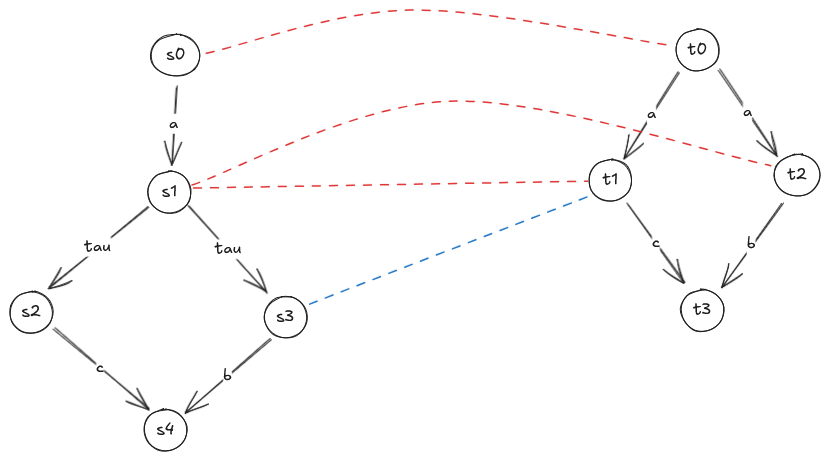
\includegraphics[width=0.7\textwidth]{02-12.png}
	\centering
\end{figure}

En particular, podemos ver que la condición de bisimulación débil nos obliga a relacionar $s_1$ con $t_1$ y $t_2$.
Por ello mismo, si nos situamos en $(s_1, t_1)$ y hacemos la transición $s_1 \overset{\tau}{\to} s_3$, la imitación deberá ser quedarse en $t_1$.
A continuación, al hacer $s_3 \overset{b}{\to} s_4$, podemos ver que en el sistema de la derecha no hay posibilidad de imitarlo.
Motivo de ello, llegamos a que es imposible tener una relación de bisimulación débil entre los dos sistemas y se concluye que es la segunda minimización (la isomorfa), la correcta respecto a la bisimulación débil.

\pagebreak
\section*{Ejercicio 13}
Se quiere ver que $P$ y $Q$ son débilmente bisimilares.
Para ello, nos vamos a basar en el siguiente diagrama:
\begin{figure}[!htb]
	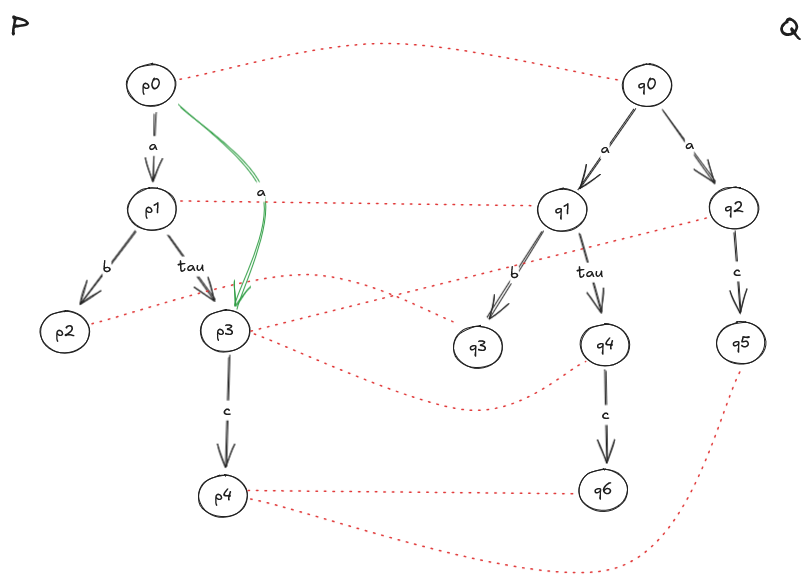
\includegraphics[width=0.7\textwidth]{02-13.png}
	\centering
\end{figure}

Gracias a este, podemos notar que la relación que lo cumple es:
\begin{equation*}
	R = \{(p_0, q_0), (p_1, q_1), (p_2, q_3), (p_3, q_4), (p_3, q_2), (p_4, q_6), (p_4, q_5)\}
\end{equation*}

\section*{Ejercicio 14}
Primero, veamos que $P$ simula a $Q$.
Para ello, nos apoyemos en el siguiente diagrama:
\begin{figure}[!htb]
	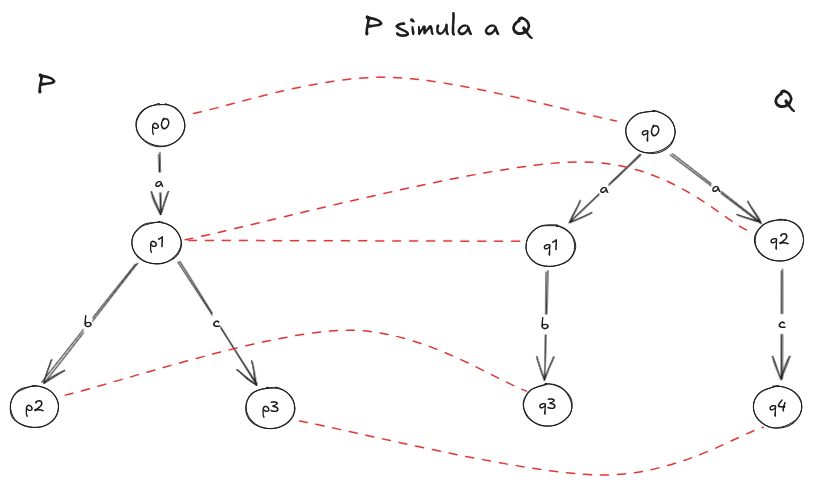
\includegraphics[width=0.7\textwidth]{02-14.png}
	\centering
\end{figure}

Gracias a él, podemos notar que $P$ simula a $Q$ bajo la relación $R = \{(q_0, p_0), (q_1, p_1), (q_2, p_1), (q_3,p_2), (q_4,p_3)\}$.

Respecto a si $Q$ simula a $P$, resulta trivial ver que no dado que al seleccionar poner ya sea a $(p_1, q_1)$ o a $(p_1, q_2)$ en la relación de equivalencia, $P$ tiene la posibilidad de elegir la transición/acción que el otro estado de $Q$ no tiene disponible.

\pagebreak
\section*{Ejercicio 15}
Para el primer punto, si queremos ver si $T$ simula a $S$, se puede considerar el siguiente diagrama:
\begin{figure}[!htb]
	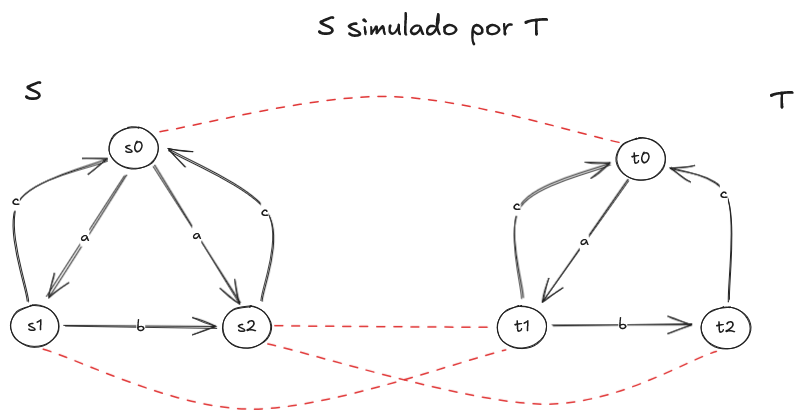
\includegraphics[width=0.8\textwidth]{02-15-a.png}
	\centering
\end{figure}

En este caso, puede verse que $R_a = \{(s_0, t_0), (s_1, t_1), (s_2, t_1), (s_2, t_2)\}$ es una simulación.

Ahora, para el segundo punto, para ver si $S$ simula a $T$, consideraremos:
\begin{figure}[!htb]
	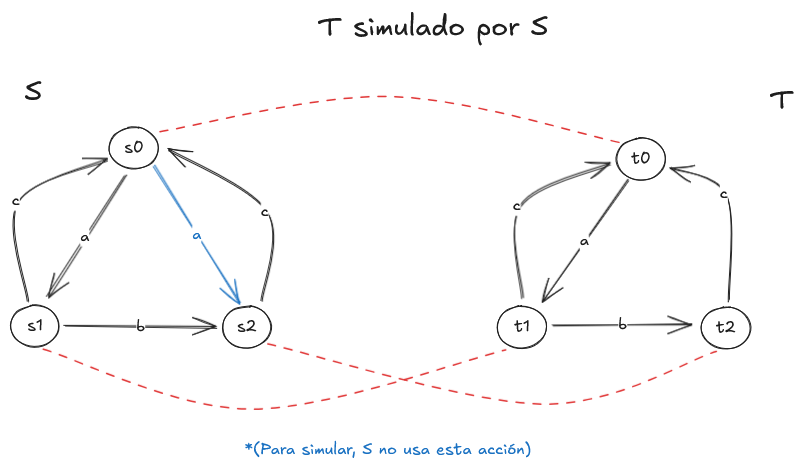
\includegraphics[width=0.8\textwidth]{02-15-b.png}
	\centering
\end{figure}

Donde $R_b = \{(t_0, s_0), (t_1, s_1), (t_2, s_2)\}$ es una relación de simulación.

Y, por último, es observable que no existe una bisimulación entre $s_0$ y $t_0$ dado que si comenzamos simulando a $S$ por $T$, estamos obligados a tener el par $(s_2, t_1)$.
Luego, si "cambiamos de rol", $t_1$ puede usar la acción $b$ cuando $s_2$ no.

\pagebreak
\section*{Ejercicio 16}
Para mayor sencillez, primero se resolverán los puntos A y C que corresponden a los sistemas $S$ y $R$, y luego se resolverá el B que corresponde a $S$ y $T$.
Respecto al primer par de sistemas, es trivial ver que no existe una bisimulación (fuerte) entre $s_0$ y $r_0$ porque este último puede realizar una acción $\tau$ mientras que $s_0$ no.
Ahora, yendo a lo interesante, que es la bisimulación débil, se considerará el siguiente diagrama:
\begin{figure}[!htb]
	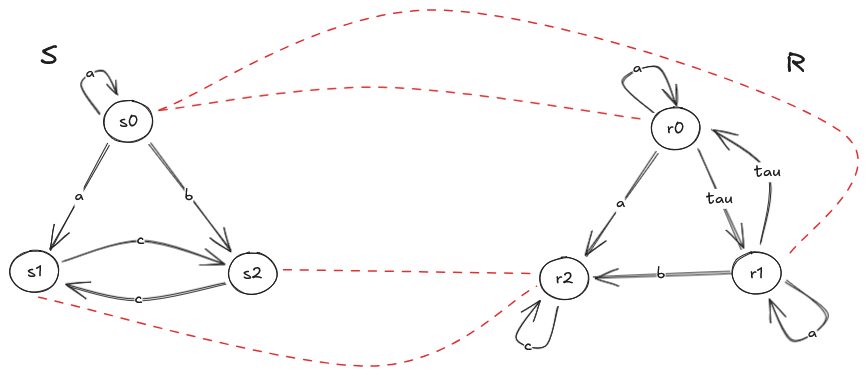
\includegraphics[width=0.8\textwidth]{02-16-c.png}
	\centering
\end{figure}

Gracias a ello, se ve que $R_c = \{(s_0, r_0), (s_0, r_1), (s_1, r_2), (s_2, r_2)\}$ es una bisimulación.

Ahora, para ver $S$ con $T$, consideramos:
\begin{figure}[!htb]
	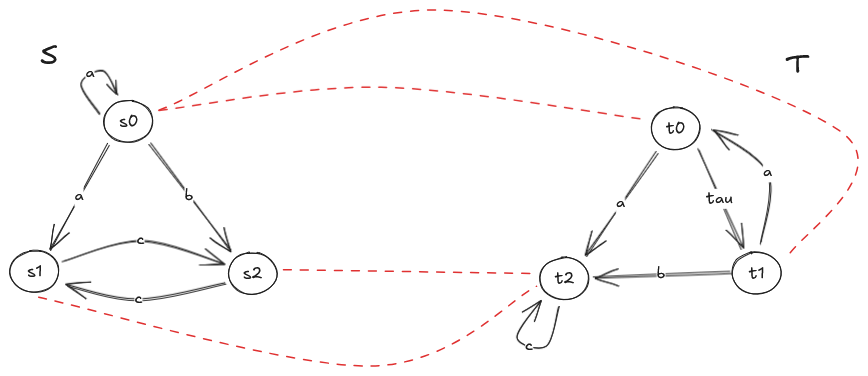
\includegraphics[width=0.8\textwidth]{02-16-b.png}
	\centering
\end{figure}

Gracias a ello, se ve que $R_b = \{(s_0, t_0), (s_0, t_1), (s_1, t_2), (s_2, t_2)\}$ es una bisimulación.

\end{document}
